\documentclass[tikz, margin=0.25mm]{standalone}

\begin{document}
    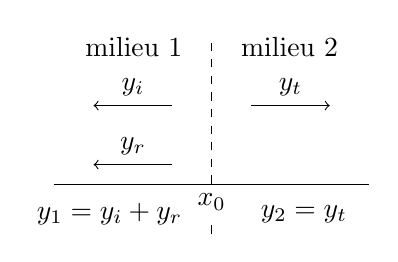
\begin{tikzpicture}
    %axis
    \node[above,left](m1) at (-.25,1.75){milieu 1};
    \node[above,right](m1) at (.25,1.75){milieu 2};
        \draw[dashed] (0,-.625) -- +(0,2.5);
        \draw[]   (-2,0) -- node[fill=white,below]{$x_0$} +(4,0) ;
    %result
    % \draw[->, red] (0,0) -- (45:1.75) node[right]{$MHS_R$};
    % \draw[] (.5,0) arc (0:45:.5) node[right]{$\theta$};
    \draw[->] (.5,1) -- node[above]{$y_t$} +(1,0);
    \draw[->] (-.5,1) -- node[above]{$y_i$} +(-1,0) ;
    \draw[->] (-.5,.25) -- node[above]{$y_r$} +(-1,0) ;
    
    \node[below,left](y1) at (-.25,-.375) {$y_1=y_i+y_r$};
    \node[below,right](y1) at (.5,-.375) {$y_2=y_t$};
    % \node[draw,below,right](ar) at (0.125,-0.5) {$a_r=A\cos(\phi)$};
    % \node[draw,above,left](br) at (-0.125,1) {$b_r=A\sin(\phi)$};
    \end{tikzpicture}  
\end{document}